\chapter{Mathematical Preliminaries}
\label{chapter:mathematical-preliminaries}

This chapter is intended to serve as a reference point, clarifying ideas and notation, for the more fundamental concepts that will be used throughout the remainder of this dissertation. In the first section we discuss order and lattice theory. The third and final section introduces propositional logic, as well more general ideas in logic.

\section{Order and Lattice Theory}
\label{section:order-theory}

This section refers extensively to the fundamental text by Davey and Priestley \cite{Davey_Priestley_2002}, as well as Ganter and Wille \cite{ganter1999formal}.

\subsection{Orders}
\label{subsection:orders}

A \textit{binary relation} \index{binary relation} $R$ over the sets $X$ and $Y$ is a set of ordered pairs $\op{x,y}$ with $x \in X$ and $y \in Y$. Alternatively, we can view $R$ as a subset of the Cartesian product of these sets, and write $R \subseteq X \times Y$. A pair $\op{x,y} \in R$ tells us that $R$ relates $x$ to $y$, and we may instead write $xRy$.

% \begin{definition}
% \label{definition:binary-relation}
% A \textit{binary relation} \index{binary relation} $R$ over two sets $X$ and $Y$ is a set of ordered pairs $\op{x,y}$ with $x \in X$ and $y \in Y$; and so $R \subseteq X \times Y$. In many cases we express this pair using infix notation, and we write $xRy$.
% \end{definition}

Certain binary relations, satisfying specific properties, occur frequently enough to warrant their own denomination. One such relation, which will be used in almost every section of this dissertation, is called a \textit{partial order}.

\begin{definition}
  \label{definition:partial-order}
  A \textit{partial-order} \index{partial-order} is a binary relation $\preceq \; \subseteq X \times X$ that satisfies the following properties:
  \begin{align}
    & \text{(Reflexivity)} & x \preceq x \\
    & \text{(Antisymmetry)} & x \preceq y \text{ and } y \preceq x \text{ implies } x = y \\
    & \text{(Transitivity)} & x \preceq y \text{ and } y \preceq z \text{ implies } x \preceq z
  \end{align}
  for all $x,y,z \in X$.
\end{definition}

Frequently, we use `preference' as a metonymy for an order; and so in the context of an order, \say{element $x$ is preferred to $y$} should be taken to mean that $\op{x,y} \in \; \preceq$, or simply $x \preceq y$.

We write $x \npreceq y$ to indicate that $\op{x,y}$ is not in the relation, and $x \prec y$ for the case where $x\preceq y$ and $x \not = y$. When $x \not \preceq y$ and $y \not \preceq x$---i.e., that $x$ and $y$ are incomparable---we write $x \Vert y$. From a partial-order we can quite easily induce the notion of a \emph{strict partial-order}.

\begin{definition}
  \label{definition:strict-partial-order}
  A \textit{strict partial-order} \index{partial-order! strict partial-order} is a binary relation $\prec \; \subseteq X \times X$ that satisfies:
  \begin{align}
    & \text{(Irreflexivity)} & x \nprec x \\
    & \text{(Asymmetry)} & x \prec y \text{ implies } y \nprec x \\
    & \text{(Transitivity)} & x \prec y \text{ and } y \prec z \text{ implies } x \prec z
  \end{align}
  for all $x,y,z \in X$.
\end{definition}

An \textit{ordered set} is a pair $(X, \preceq)$ with $X$ being a set and $\preceq$ being an ordering on $X$, we use bold-face as a shorthand, and so $\mathbf{X}$ is an ordered set, and the order relation associated with $\mathbf{X}$ may be written $\preceq_X$ if there is ambiguity. If $\mathbf{Y}$ is a subset of $\mathbf{X}$, then $\mathbf{Y}$ inherits the order relation from $\mathbf{X}$; and so, for $x,y \in \mathbf{Y}$, $x \preceq_Y y$ if and only if $x \preceq_X y$.

We can visualise ordered sets through the use of \textit{Hasse} diagrams\index{Hasse diagrams}.

\begin{figure}[H]
  \centering
  \small
  \begin{subfigure}{0.3\textwidth}
    \centering
    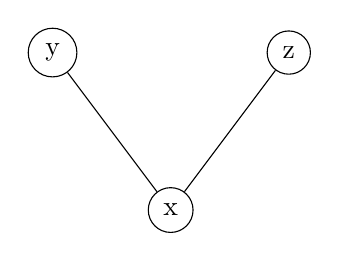
\begin{tikzpicture}[every node/.style={circle, draw, minimum size=0.25cm}]
      \node (y) at (-1.5,0) {y};
      \node (z) at (1.5,0) {z};
      \node (x) at (0,-2) {x};

      \draw (y) -- (x);
      \draw (z) -- (x);
    \end{tikzpicture}
    \subcaption{$\mathbf{A}$}
    \label{subfigure:partial-order-a}
  \end{subfigure}%
  \begin{subfigure}{0.3\textwidth}
    \centering
    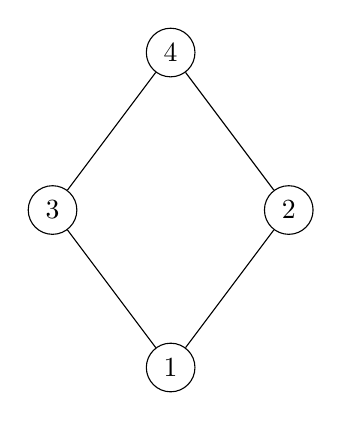
\begin{tikzpicture}[every node/.style={circle, draw, minimum size=0.25cm}]
      \node (w) at (0,2) {4};
      \node (y) at (-1.5,0) {3};
      \node (z) at (1.5,0) {2};
      \node (x) at (0,-2) {1};

      \draw (w) -- (y);
      \draw (w) -- (z);
      \draw (y) -- (x);
      \draw (z) -- (x);
    \end{tikzpicture}
    \subcaption{$\mathbf{B}$}
    \label{subfigure:partial-order-b}
  \end{subfigure}%
  \begin{subfigure}{0.3\textwidth}
    \centering
    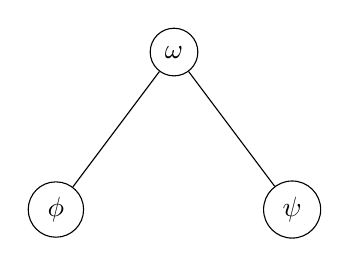
\begin{tikzpicture}[every node/.style={circle, draw, minimum size=0.25cm}]
      \node (y) at (-1.5,0) {$\phi$};
      \node (z) at (1.5,0) {$\psi$};
      \node (x) at (0,2) {$\omega$};

      \draw (y) -- (x);
      \draw (z) -- (x);
    \end{tikzpicture}
    \subcaption{$\mathbf{C}$}
    \label{subfigure:partial-order-c}
  \end{subfigure}%
  \caption{Three partial-orders over a set $P$}
  \label{figure:hasse-diagram}
\end{figure}

Then, a pair $\op{x,y}$ is in a given order relation $\preceq \; \subseteq X \times X$ if there exists a strictly upward path connecting $x$ to $y$ (or, if $x = y$). From $\mathbf{C}$ we can read-off that $\phi || \psi$, and that $\phi \preceq_C \omega$, for instance.
%For the inverse of an order $\preceq$ we write $\preceq^{-1}$, and so in \Cref{figure:hasse-diagram} $\preceq_\mathbf{A}^{-1} = \preceq_\mathbf{C}$ \cite{ganter1999formal}.

\begin{definition}
  \label{definition:order-maps}
  \index{order preserving map} \index{isotone function} \index{order-isomorphism}
  Let $\mathbf{X}$ and $\mathbf{Y}$ be ordered sets with a map $\varphi : \mathbf{X} \to \mathbf{Y}$. We say that $\varphi$ is an \textit{order-preserving} (or, isotone) map if $x \preceq_X y$ implies $\varphi(x) \preceq_Y \varphi(y)$. It is an \textit{order-embedding} if it is injective, and $x \preceq_X y$ if and only if $\varphi(x) \preceq_Y \varphi(y)$ for all $x,y \in X$. Finally, $\varphi$ is an \textit{order-isomorphism} if it is an order-embedding that is also \textit{onto}.
\end{definition}

An order-mapping is called \textit{antitone} if it reverses the order and is the dual to isotone mappings, where \textit{antitone order-embeddings} and \textit{antitone order-isomorphisms} are defined as one might expect. In \Cref{figure:hasse-diagram} it is quite simply to find an antitone order-isomorphism between $\mathbf{A}$ and $\mathbf{C}$. \index{antitone function}

If $\mathbf{X}$ is an ordered set, then an element $x \in X$ is \textit{minimal} in $\mathbf{X}$ if there exists no distinct element $y \in X$ such that $y \preceq x$. Conversely, $x$ is \textit{maximal} in $\mathbf{X}$ if there exists no distinct $y \in X$ with $x \preceq y$. Continuing this example, $x$ is the \textit{minimum} of $\mathbf{X}$ if it is minimal in $\mathbf{X}$ and there are no elements to which $x$ is incomparable. In other words, for every element $y \in X$ it is the case that $x \preceq y$. Naturally, $x$ is the \textit{maximum} element of $\mathbf{X}$ if for all $y \in X$ it is the case that $y \preceq x$.

\begin{definition}
  \label{definition:infimum-supremum}
  Let $(X,\preceq)$ be a partially ordered set, and $\mathbf{Y}$ a subset of $\mathbf{X}$. The \textit{lower bound} of $\mathbf{Y}$ is an element $x \in X$ with $x \preceq y$ for all $y \in Y$. The \textit{upper bound} of $Y$ is defined dually. If the set of lower bounds of $Y$ has a maximum (greatest) element then this element is called the \textit{infimum} of $Y$. Dually, if there is a minimum (least) element in the set of upper bounds, then this element is the \textit{supremum} of $Y$.
  \index{supremum} \index{infimum}
\end{definition}

\begin{remark}
  \label{remark:natural-order-subset-inclusion}
  For any set $X$, the power-set of $X$ equipped with an order determined by subset inclusion will form a partial order. Then, $(2^X, \preceq)$ is a partially ordered set where for two sets $A, B \in 2^X$ where $A \preceq B$ if and only if $A \subseteq B$. It follows that $\mathbf{X}$ will always have a minimum: $\emptyset$, and a maximum: $X$.
\end{remark}

\subsection{Lattices}
\label{subsection:lattices}
\index{lattices}

One perspective, which we adopt, views a \textit{lattice} as a particular kind of partially ordered set satisfying specific properties involving upper and lower bounds. In particular,

\begin{definition}
  \label{definition:complete-lattice}
  A partially ordered set $\mathbf{X} = (X, \preceq)$ is a \textit{lattice} if and only if, for any two elements $x, y \in \mathbf{X}$, both the supremum $x \vee y$ and the infimum $x \wedge y$ exist. The set $\mathbf{X}$ is a \textit{complete lattice} if and only if the meet and join exist for every subset of $\mathbf{X}$.
\end{definition}

In \Cref{figure:hasse-diagram} only (b) is a lattice (and a complete lattice too). In fact, every finite lattice is a complete lattice \cite{ganter1999formal}.

\section{Propositional Logic}
\label{section:propositional-logic}
